\section{The vertical $\sigma$-coordinate}
\label{Scoord}

ROMS now supports several vertical coordinate systems as fully
described on the
\href{https://www.myroms.org/wiki/index.php/Vertical_S-coordinate}{ROMS
wiki}. See also \cite{SS2005}. The
currently recommended values correspond to \code{Vtransform}$=2$
and \code{Vstretching}$=4$, therefore that is what is described here.

\subsection{Transform}
The vertical coordinate corresponding to \code{Vtransform}$=2$ is:
\begin{equation}
     z(x,y,\sigma,t) = \zeta(x,y,t) + \left[\zeta(x,y,t) +
     h(x,y)\right] \, S(x,y,\sigma),
\end{equation}
\begin{equation}
     S(x,y,\sigma) = \frac{h_c \, \sigma + h(x,y)\,
          C(\sigma)}{h_c + h(x,y)}
\end{equation}
where $h_c$ is a (positive) thickness above
which we wish to have more resolution and $C(\sigma)$ is a
nondimensional, monotonic, vertical
stretching function ranging from $-1 \le C(\sigma) \le 0$.

In an undisturbed ocean state, corresponding to zero free-surface,
$z=S(x,y,\sigma)$ so that in our coordinate system, the depths are not
affected by the displacements of the free-surface.  This ensures that
the vertical mass fluxes generated by a purely barotropic motion will
vanish at every interface.

%where $\theta$ and $b$ are surface and bottom control parameters.
%Their ranges are $0 < \theta \leq 20$ and $0 \leq b \leq 1$,
%respectively.  Equation (\ref{zetaa}) leads to $z = \zeta$ for
%$\sigma = 0$ and $z = h$ for $\sigma = -1$.

%Some features of this coordinate system:
%\begin{itemize}
%   \item It is a generalization of the traditional $\sigma$-coordinate
%   system.  Letting $\theta$ go to zero and using L'Hopital's rule,
%   we get:
%   \begin{equation}
%      z = (\zeta + h)(1 + \sigma) - h
%   \end{equation}
%   which is the classic $\sigma$-coordinate.
%   \item It is infinitely differentiable in $\sigma$.
%   \item The larger the value of $\theta$, the more resolution is kept
%   above $h_c$.
%   \item For $b = 0$, the resolution all goes to the surface as
%   $\theta$ is increased.
%   \item For $b = 1$, the resolution goes to both the surface and the
%   bottom equally as $\theta$ is increased.
%\end{itemize}
%Figure \ref{fscd} shows the $\sigma$-surfaces for several values of $\theta$
%and $b$ for one of our domains.  It was produced by a Matlab tool
%written by Hernan Arango which is available from our web site (see
%\S\ref{Myroms}).

%\begin{figure}
%\setlength{\unitlength}{10mm}
%\begin{picture}(0,18)(0,0)
%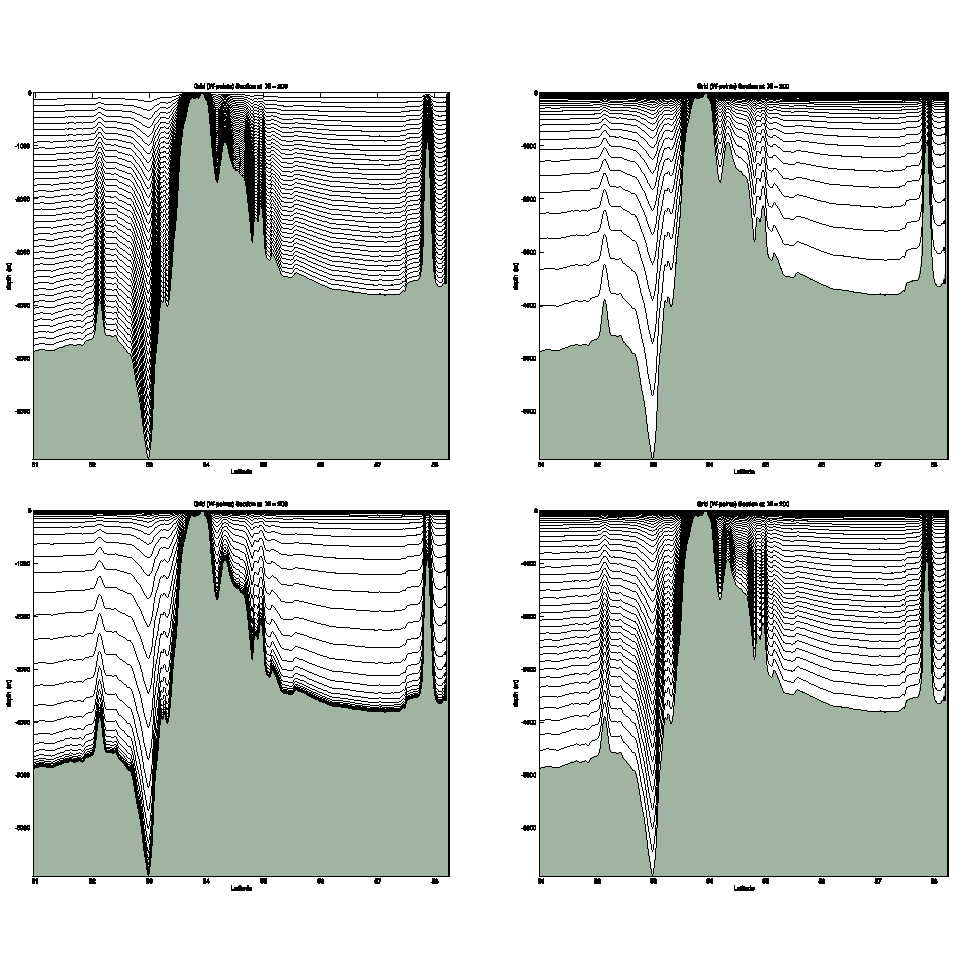
\includegraphics{pics/scoord}
%\end{picture}
%
%\caption{The $\sigma$-surfaces for the North Atlantic with (a) $\theta =
%0.0001$ and $b = 0$, (b) $\theta = 8$ and $b = 0$, (c) $\theta = 8$
%and $b = 1$.  (d) The actual values used in this domain were
%$\theta = 5$ and $b = 0.4$.}
%\label{fscd}
%\end{figure}

We find it convenient to define:
\begin{equation}
   H_z \equiv {\partial z \over \partial \sigma}
\end{equation}
We compute $H_z$ discretely as $\Delta z/ \Delta
\sigma$ since this leads to the vertical sum of $H_z$ being exactly the
total water depth $D$.

Notice that, unlike our previous stretching function,
\begin{equation}
  S(x,y,\sigma) = \left\{ \begin{array}{lll}
       0,  &\mbox{if $\;\;\sigma = \phantom{-}0,
 \;\; C(\sigma) = \phantom{-}0$,} & \mbox{at the free-surface;} \\
       -1,  &\mbox{if $\;\;\sigma = -1, \;\;
	    C(\sigma) = -1$,} & \mbox{at the ocean bottom;}
	    \end{array} \right.
\end{equation}
The new stretching is superior in that:
\begin{itemize}
   \item Regardless of the design of $C(\sigma)$, it behaves like
   equally-spaced sigma-coordinates in shallow regions, where
   $h(x,y) \ll h_c$.  This is advantageous because it avoids
   excessive resolution and associated CFL limitation is such areas.

   \item Near-surface refinement behaves more or less like geopotential
   coordinates in deep regions (level thicknesses, $H_z$, do not
   depend or weakly depend on bathymetry), while near-bottom like
   sigma coordinates ($H_z$ is roughly proportional to depth).
   This reduces the extreme r-factors near the bottom and reduces
   pressure gradient errors.

   \item The ``true'' sigma-coordinate system is recovered as $h_c
   \rightarrow \infty$. This is useful when configuring
   applications with ``flat'' bathymetry and ``uniform'' level
   thickness.  Practically, you can achieve this by setting
   \code{Tcline} to 1.0d+16 in \code{ocean.in}.
   This will set $h_c=1.0\hbox{x}10^{16}$. Although not necessary,
   we also recommend that you set $\theta_S=0$ and
   $\theta_B=0$.

   \item In an undisturbed ocean state, $\zeta\equiv 0$,
   transformation (2) yields the following unperturbed depths, $\hat{z}$,
\begin{equation}
   \hat{z}(x,y,\sigma) \equiv h(x,y) \, S(x,y,\sigma) = h(x,y)
   \left[\frac{h_c \, \sigma + h(x,y)\, C(\sigma)}{h_c +
   h(x,y)}\right]
\end{equation}
   and
\begin{equation}
   d\hat{z} = d\sigma \; h(x,y) \; \left[\frac{h_c}{h_c +
   h(x,y)}\right]
\end{equation}
   As a consequence, the uppermost grid box retains very little
   dependency from bathymetry in deep areas, where $h_c \ll h(x,y)$.
   For example, if $h_c = 250\,m$ and $h(x,y)$ changes from $2000$
   to $6000\,m$, the uppermost grid box changes only by a factor
   of 1.08 (less than $10\%$).
\end{itemize}

\subsection{Stretching}
In ROMS, we recommend \code{Vstretching}$ = 4$. $C(\sigma)$ is defined as
a continuous, double stretching function: 
\begin{itemize}
   \item Surface refinement function: 
\begin{equation}
C(\sigma) = \frac{1 -
\cosh(\theta_S \, \sigma)}{\cosh(\theta_S) - 1}, \qquad  \mbox{for
}\theta_S > 0, \qquad C(\sigma) = -{\sigma}^{2}, \qquad \mbox{for
}\theta_S \le 0
\label{eqctop}
\end{equation}
  \item Bottom refinement function:
\begin{equation}
C(\sigma) = \frac
{\exp(\theta_B\,C(\sigma)) - 1} {1 - \exp(-\theta_B)}, \qquad
\mbox{for }\theta_B > 0
\label{eqcbot}
\end{equation}
\end{itemize}
Notice that the bottom
function (\ref{eqcbot}) is the second stretching of an already
stretched transform (\ref{eqctop}). The resulting stretching
function is continuous with respect to $\theta_S$ and $\theta_B$ as
their values approach zero. The range of meaningful values for
$\theta_S$ and $\theta_B$ are:
$$ 0 \le \theta_S \le 10
\qquad \hbox{and} \qquad 0 \le \theta_B \le 4
$$
However, users need to pay attention to extreme r-factor \code{rx1}
values near the bottom.
